\newpage
\section{Properties of Harmonic Functions}

\subsection{Elliptic regularity}
Recall that if we have the Laplace equation
$$
-\Delta u=f \quad \text { in } \mathbb{R}^{n}
$$
then we have the fundamental solution
$$
K(x)= 
\begin{cases}
    \frac{c_{n}}{|x|^{2-n}} & n \geq 3 \\ 
    \frac{1}{2 \pi} \ln |x| & n=2,
\end{cases}
$$

and we can get a solution $u=K * f$. However, there are a number of questions we have not answered, such as uniqueness of solutions.

\begin{definition}
    [Harmonic]
    A function such that $-\Delta u = 0$ is called harmonic.
\end{definition}

\begin{theorem}
    [Elliptic regularity]
    Harmonic functions are smooth.
\end{theorem}

That is, if we have a local solution $u \in \mathcal{D}^{\prime}$, we want to show that $u \in C^{\infty}$. Why should harmonic functions be smooth? This is because the fundamental solution $K$ is smooth away from 0 . Let's see how the reasoning goes.

\vspace{1em}
\begin{proof}
    Let $\Omega$ be the domain where $u$ lives. Choose a point $x_{0} \in \Omega$, and we want to show that $u$ is smooth around $x_{0} .$ Draw a ball $B$ around $x_{0}$ and a larger ball $2 B$ around $B$. To use the fundamental solution, chop off $u$ by using a cutoff function
    \[
        \chi(x)= \begin{cases}1 & x \in B \\ \text { smooth } & x \in 2 B \backslash B \\ 0 & x \in 2 B^{c}\end{cases}
    \]
    \begin{figure}[H]
        \centering
        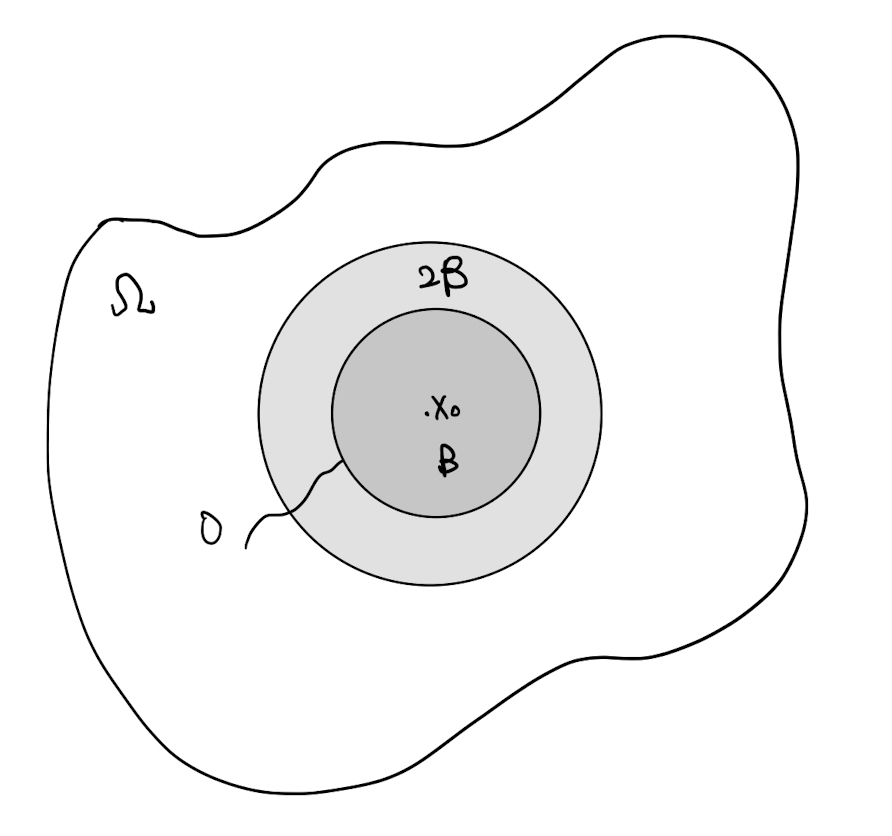
\includegraphics[width=0.5\textwidth]{pics/22-1.png}
    \end{figure}
    If we let $v=\chi u$, then
$$
-\Delta v=\underbrace{-\chi \Delta u}_{=0}-u \Delta \chi-2 \nabla u \cdot \nabla \chi
$$
This gives us the new problem
$$
-\Delta=f, \quad f \in \mathcal{D}^{\prime}, \quad \operatorname{supp} f \subseteq 2 B \backslash B
$$
Then
$$
\begin{aligned}
v(x) &=(K * f)(x) \\
&=\int K(x-y) f(y) d y
\end{aligned}
$$
Suppose we want a local solution in, say, $B / 2$, where $B$ has radius $R$. If $x \in B / 2$ and $y \in 2 B \backslash B$, then $|x-y| \geq r / 2 .$ Now $K(z)$ is smooth where $|z| \geq r / 2$, which means this convolution is smooth for $x \in B / 2$.
\qed 
\end{proof}

\begin{remark}
    ~\
    \begin{itemize}
        \item We didn't use much about the Laplace equation itself here. We only used the fact that $K$ is smooth away from 0.
        \item This is not all there is to elliptic regularity. $K$ is analytic away from $0$, which tells us that $u$ is analytic.
        \item More generally, we may want to make statements about what kind of regularity $u$ has if $f$ has a certain degree of regularity. This is what elliptic regularity really is, and this is only the tip of the iceberg.
    \end{itemize}
\end{remark}

\subsection{The maximum principle}

\begin{definition}
[subharmonic, superharmonic]
A function $u$ such that $-\Delta u \le 0$ is called subharmonic. A fuction $u$ such that $-\Delta u\ge 0$ is called superharmonic.
\end{definition}
We will prove results for harmonic functions and claim that they hold for sub and superharmonic functions, as well.

Suppose $-\Delta u=0$ in $\Omega$. Where is the $\max / \min$ of $u$ ? The first step to answering this question is to look at the \textbf{mean value property}.

\begin{theorem}
[Mean value property]
Suppose $-\Delta u = 0$ in $B(x_0,a)$. Then
\[
    \begin{aligned}
        u\left(x_{0}\right) &=\frac{1}{|B|} \int_{B} u(x) d x =\frac{1}{|\partial B|} \int_{\partial B} u(x) d \sigma,
        \end{aligned}
\]
where $\sigma$ is surface measure on the sphere $\partial B$.
\end{theorem}

\begin{remark}
    If we assume $u$ is subharmonic, i.e. $-\Delta u\le 0$, then we get $\le$ instead of equalities. The reverse inequality holds for superharmonic functions.
\end{remark}

\begin{lemma}
    [Green's theorem]
     Suppose $u: \Omega \rightarrow \mathbb{R} .$ Then
$$
\int_{\Omega} \partial_{j} u d x=\int_{\partial \Omega} u \cdot \nu_{j} d \sigma
$$
where $\nu_{j}$ is the outward pointing normal to $\partial \Omega .$ Equivalently,
$$
\int \underbrace{\partial_{j} u_{j}}_{\operatorname{div} u} d x=\int_{\partial \Omega} u \cdot \nu d \sigma
$$
\end{lemma}
Here's how we can use this: Integrating by parts twice in the following integral keeps the sign the same and introducing 2 boundary terms:
\[
    \int_\Omega \Delta u \cdot v d x-\int_{\Omega} u \cdot \Delta v d x=\int_{\partial \Omega} \underbrace{\partial_{j} u \nu_{j}}_{\frac{\partial u}{\partial \nu}} \cdot v-u \cdot \underbrace{\nu_{j} \partial_{j} v}_{\frac{\partial v}{\partial \nu}} d \sigma,
\]
where these $\nu$ are normal derivatives. Now let's prove the mean value property:
\vspace{1em}
\begin{proof}
     Suppose $B=B(0, r)$, and apply Green's theorem with a well-chosen $v$. Looking at our equation, it would be nice if we could make $v=0$ on the boundary. So we can try
$$
v=K(|x|)-K(r).
$$
We get
$$
u(0)=c \int_{\partial B} u d \sigma .
$$
This holds for all harmonic functions. If we set $u=1$, then we get $c=\frac{1}{\mid \frac{1}{|B|} \text {, so } u=}$ $\frac{1}{\partial B \mid} \int_{\partial B} u$.
\qed
\end{proof}

\begin{corollary}
    If $u(x_0)= \max u$ for $x_0\in B$, then $u$ is constant in $B$.
\end{corollary}
\begin{remark}
    If $u$ is subharmonic, the same holds. But if $u$ is superharmonic, then we need to replace the maximum with the minimum in this property.
\end{remark}


\begin{theorem}
    [Strong maximal principle]
    Suppose $u \in C^{2}(\Omega) \cap C(\bar{\Omega})$ is harmonic. Then $\max _{\bar{\Omega}} u=\max _{\partial \Omega} u$
Moreover, if $\max u$ is attained inside $\Omega$, then $u$ is constant.
\end{theorem}

\begin{proof}
    If $\max u$ is only attained on $\partial \Omega$, then we ar edone. What if $\max u$ is attained at $x_{0} \in \Omega ?$ Here is a proof by picture. Put a ball around $x_{0} .$ By the corollary, $u$ is constant in $B$. Then the other points in this ball are maximum points, and we can get to any other point via a sequence of balls.

    \begin{figure}[H]
        \centering
        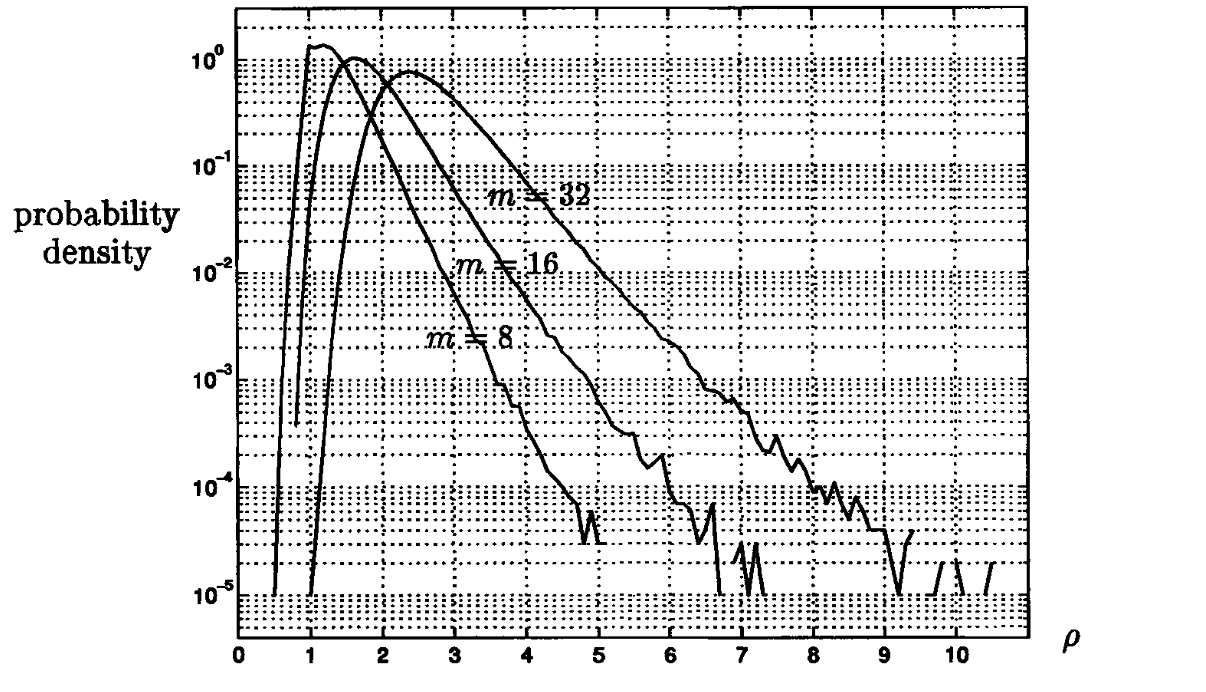
\includegraphics[width=0.4\textwidth]{Pics/22-2.png}
    \end{figure}
    If you want to write down a proof, you can use path-connectedness, or you can use an argument like this: Let $A=\left\{x \in \Omega: u(x)=u\left(x_{0}\right)\right\} .$ Since $u$ is continuous, $A$ is closed. But the corollary says that if $x_{0} \in A$, then $B\left(X_{0}, r\right) \subseteq A .$ So $A$ is open. Thus, $A \subseteq \Omega$ is open and closed, and if $\Omega$ is connected, we get $A=\Omega$.
    \qed 
\end{proof}
\begin{remark}
    If $u$ is subharmonic, the same holds. But if $u$ is superharmonic, then we need to replace the maximum with the minimum in this property. Besides, the hypotheses here are much stronger than they need to be.
\end{remark}

\begin{corollary}
    [Comparison principle]
    Let $u$ be subharmonic, i.e., $-\Delta u \leq 0$, and let $v$ be subharmonic, i.e., $-\Delta v \geq 0$. If $u \leq v$ on $\partial \Omega$, then $u \leq v$ in $\bar{\partial} \Omega$.
\end{corollary}

This comparison principle is the correct statement for nonlinear elliptic stuff and also for the Hamilton-Jacobi equations. There is a simpler proof of the maximum principle without the use of the fundamental solution where we drop the strong part.

\vspace{1em}
\begin{proof}
Suppose first that $-\Delta u<0 .$ Let $x_{0}$ be a maximum point inside $\Omega .$ Then $\nabla u\left(x_{0}\right)=$ 0, and $H u\left(x_{0}\right) \prec 0$, where $H=\frac{\partial^{2} u}{\partial x_{i} \partial x_{j}}$ is the Hessian matrix. Observe that
$$
\Delta u=\sum_{j} \partial_{j} \partial_{j} u=\operatorname{tr} H u \leq 0
$$
Then $\Delta u\left(x_{0}\right) \leq 0$, so $-\Delta u\left(x_{0}\right) \geq 0 .$ But this contradicts our assumption that $-\Delta u<0$ Now if $-\Delta u \leq 0$, then we penalize $u$ by replacing $u$ by $u_{\varepsilon}=u+\varepsilon x^{2} .$ Then
$$
-\Delta u_{\varepsilon}=-\Delta u-2 u \varepsilon<0
$$
This tells us that
$$
\max _{\bar{\Omega}} u_{\varepsilon}=\max _{\partial_{\Omega}} u_{\varepsilon}
$$
If we let $\varepsilon \rightarrow 0$, both sides converge uniformly to $\max _{\bar{\Omega}} u$ and $\max _{\partial \Omega} u$, respectively.
\end{proof}

\subsection{Liouville's thoerem}
We have been looking at harmonic functions in a domain $\Omega$. What if we are looking at harmonic functions in all of $\mathbb{R}^{n} ?$ If you allow exponential growth, then the sky is the limit as to what you can get. But what if we only want polynomial growth. Further yet, what if $u$ is bounded?

\begin{theorem}
    [Liouville]
    Let $u$ be harmonic in $\RR^n$. If $u$ is bounded, then $u$ is constant.
\end{theorem}
\begin{proof}
    If $u$ is harmonic, so are its derivatives. Then
$$
\begin{aligned}
\partial_j u\left(x_{0}\right) & \stackrel{\text { MVP }}{=} \int_{\Omega} \partial_{j} u(x) d x \\
&=\frac{1}{\left|B_{R}\right|} \int_{\partial B_{R}} u \cdot \nu_{j} d \sigma(x)
\end{aligned}
$$
If $|u| \leq M$, we can estimate this by
$$
\begin{aligned}
\left|\partial_{j} u\left(x_{0}\right)\right| & \leq \underbrace{\frac{1}{B_{R}}}_{R^{n}} M \underbrace{\left|\partial B_{R}\right|}_{R^{n-1}} \\
& \lesssim \frac{M}{R} \\
& \stackrel{R \rightarrow \infty}{\longrightarrow} 0
\end{aligned}
$$
So $\nabla u\left(x_{0}\right)=0$, which means that $u$ is constant.
\qed 
\end{proof}

\begin{remark}
    If $u$ is temperate, then $\hat{u}\|\xi\|^2 = 0$, so $\hat u$ is supported at $0$. Then $\hat u = \sum_{\alpha}c_\alpha \delta_0^{(\alpha)}$, which implies that $u$ is a polynomial. Thus, all temperate harmonic functions are polynomials. This also serves as a proof of Liouville's theorem, since the only polynomials are constant.
\end{remark}

\subsection{Boundary value problem}
Let $\Omega \subset \RR^n$, and suppose that
\[
    \begin{cases}-\Delta u=f & \text { in } \Omega \\ u=g & \text { on } \partial \Omega\end{cases}.
\]
This give us uniqueness: Suppose $u_{1}, u_{2}$ are solutions. If $u_{1}-u_{2}=v$, then $v$ is harmonic. The maximum and minimum principles give
$$
\begin{aligned}
&\max _{\Omega} v \leq \max _{\partial \Omega} v=0 \\
&\min _{\Omega} v \geq \min _{\partial \Omega} v=0
\end{aligned}
$$
So $v=0$.
There is also a proof of existence using hte maximum principle. Consider a subsolution $v^{-}$satisfying
$$
\left\{\begin{array}{l}
-\Delta v^{-} \leq f \\
v \leq g
\end{array}\right.
$$
and a supersolution satisfying
$$
\left\{\begin{array}{l}
-\Delta v^{+} \geq f \\
v \geq g
\end{array}\right.
$$
The maximum principle $v^{+} \geq v^{-}$. Taking the maximum over all supersolutions and subsolutions gives the largest subsolution and the smallest supersolution.

\begin{figure}[H]
    \centering
    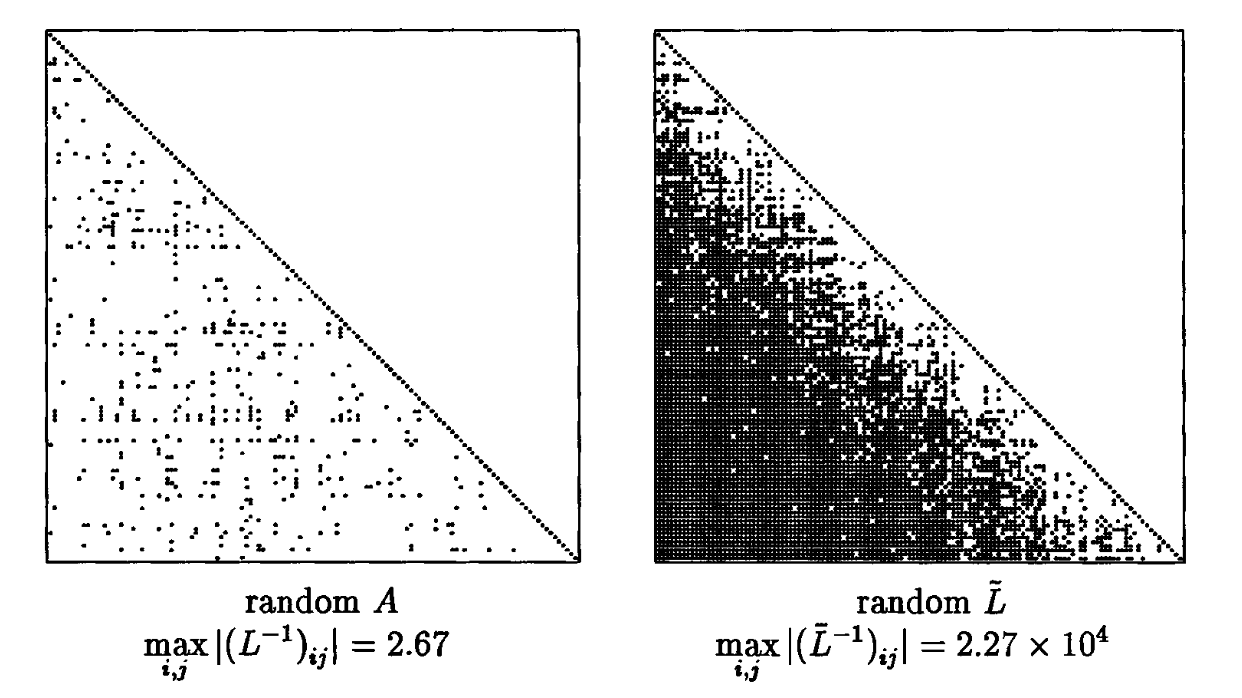
\includegraphics[width=0.3\textwidth]{Pics/22-3.png}
\end{figure}
This is called Perron's method. We can also find a fundamental solution in $\Omega$, called a Green function.